%!LW recipe=pdflatex -> bibtex -> pdflatex -> pdflatex
\documentclass[conference, letterpaper]{IEEEtran}
\usepackage{cite}
\usepackage{amsmath,amssymb,amsfonts}
\usepackage{algorithmic}
\usepackage{graphicx}
\usepackage{textcomp}
\usepackage{xcolor}
\usepackage{blindtext}
\usepackage{booktabs}
\usepackage{bm}
\usepackage[none]{hyphenat}

\def\BibTeX{{\rm B\kern-.05em{\sc i\kern-.025em b}\kern-.08em
    T\kern-.1667em\lower.7ex\hbox{E}\kern-.125emX}}
\begin{document}

\title{Generation of a Calibration for a Load Cell}

\author{\IEEEauthorblockN{Jamie Kang}}

\maketitle

\section{Introduction}
    Load cells measure mechanical force by converting applied force into an electrical signal. The load cell used during this lab uses a strain gauge attached to a metal bar to translate the strain formed in the material of the bar from the stress caused by the force applied into output voltage, which is then displayed on the screen of the strain gauge amplifier. In order to relate the value displayed on the screen to the force applied to the load cell, a calibration function is needed. \par
    \smallskip
    This lab goes through the process of applying known forces to the load cell and using statistical methods to generate said calibration function from the corresponding outputs. As the applied force increases, the output displayed on the strain gauge amplifier is expected to increase proportionally, resulting in a linear calibration curve.

\section{Materials and Methods}
    Equipment and procedures from the lab 1 manual\cite{1OLM2023} provided was used to generate calibration data from hanging 100g, 200g, 500g, 700g, 1000g, 1200g, and 1500g masses on the load cell. 
    Formulations from Statistical Methods by Snedecor and Cochran\cite{SNEDECOR1989} were used to calculate the mean, standard deviation, regression, and coefficient of determination from the obtained data; the regression and coefficient of determination were plotted using MATLAB.\@

\section{Results}
    \vspace*{-\baselineskip}
    \begin{figure}[htbp]
    \centerline{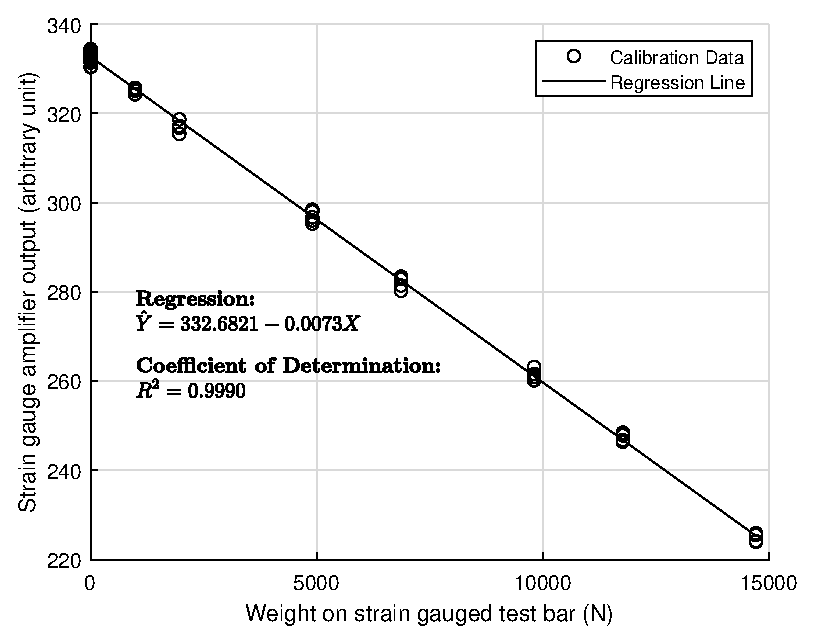
\includegraphics[width = \linewidth]{lab1fig.eps}}
    \caption{Calibration data generated and its linear regression line plotted on graph relating weight applied to strain gauged test bar with strain gauge amplifier output. The equation of the regression line and the coefficient of determination is shown alongside.}\label{fig}
    \end{figure}
    \vspace*{-\baselineskip}
    \begin{table}[htbp]
        \caption{Mean Output and Its Standard Deviation for Calibration Data per Each Calibration Mass / Weight Used in Arbitrary Units}
        \centering
        \begin{tabular}{cccc}
            \toprule{}
            \textbf{Mass (\(\bm{g}\))} & \textbf{Weight (\(\bm{N}\))} & \textbf{Mean Output} & \textbf{Standard Deviation}\\
            \midrule{}
            100 & 981 & \(324.9380\) & \(0.6175\) \\
            200 & 1962 & \(317.0360\) & \(1.1624\) \\
            500 & 4905 & \(296.9040\) & \(1.3129\) \\
            700 & 6867 & \(282.2480\) & \(1.3506\) \\
            1000 & 9810 & \(261.2520\) & \(1.2312\) \\
            1200 & 11772 & \(247.5380\) & \(0.8949\) \\
            1500 & 14715 & \(225.0820\) & \(0.9141\) \\
            \bottomrule{}
        \end{tabular}\label{tab1}
    \end{table}
    \vspace*{-\baselineskip}

\section{Discussion}
The strain gauge amplifier's output decreases as more downward force is applied to the test bar, indicating that the strain gauge measures compressive strain when subjected to downward flexion. This contradicts the initial hypothesis which assumed tensile strain would be measured leading to an incorrect expectation of a proportional increase in output; the magnitude of the difference between the output for the zero-load value and the force tested increased, not the raw output. \par
\smallskip
The high coefficient of determination \((R^2 = 0.9990)\) for the calibration function suggests an excellent fit between the collected data and the calibration curve, ensuring the load cell's reliability within the 0--14715N downwards applied force range. Some deviations in the data may have been caused by adjusting the test bar during data collection and incomplete settling of calibration weights before data collection. \par
\smallskip
Measuring forces outside of the 0--14715N downwards applied force range reduces load cell reliability. When forces cause upward flexion, the strain gauge measures tensile strain, resulting in a positive value for the difference between the output for the zero-load value and the force tested. The calibration function, generated solely with downward flexion tests, may not accurately represent sensor behavior for upward flexion. \par
\smallskip
Lastly, clarification is needed for the terms ``calibration mass'' and ``calibration weight.'' While both terms are used, it's more accurate to refer to them as calibration weights, as the load cell ultimately deals with force rather than mass. \par

\bibliographystyle{ieeetran}
\bibliography{lab1}

\end{document}